
%%%%%%%%%%%%%%%%%%%%%%%%%%%%%%%%%%%%%%%%%%%%%%%%%%%%%%%%%%%%%%%%%%%%%%%%%%%%%
%%%%% Pointers %%%%%%%%%%%%%%%%%%%%%%%%%%%%%%%%%%%%%%%%%%%%%%%%%%%%%%%%%%%%%%
%%%%%%%%%%%%%%%%%%%%%%%%%%%%%%%%%%%%%%%%%%%%%%%%%%%%%%%%%%%%%%%%%%%%%%%%%%%%%
\begin{frame}
\pointedsl{
	Pointers
}
\end{frame}

%%%%%%%%%%%%%%%%%%%%%%%%%%%%%%%%%%%%%%%%%%%%%%%%%%%%%%%%%%%%%%%%%%%%%%%%%%%%%
\begin{frame}[fragile]
\frametitle{Passing by value}
\begin{lstlisting}
void swap_wrong(int x, int y){
    int tmp = x;
    x = y;
    y = tmp;
}
int a = 1, b = 2;
swap_wrong(a, b);
// did not work! a=1, b=2
\end{lstlisting}
\misc{
	Function arguments are \textbf{passed by value} (copy of value). We need pointers to modify \ctext{a} and \ctext{b} in the code above.
}
\end{frame}

\begin{frame}[fragile]
\frametitle{Using pointers}
\begin{lstlisting}
void swap_ptr(int *x, int *y){
    int tmp = *x;
    *x = *y;
    *y = tmp;
}
int a = 1, b = 2;
swap_ptr(&a, &b);
// now a=2, b=1
\end{lstlisting}
\misc{
	\ctext{\&a} uses the \textbf{reference} operator to get the adresse of \ctext{a}.
	
	\ctext{*x} uses the \textbf{dereference} operator to get / set the value at the adress given by \ctext{x}.
}
\end{frame}

\begin{frame}[fragile]
\frametitle{References}
\begin{lstlisting}
// passed by reference
void swap_ref(int &x, int &y){
    int tmp = x;
    x = y;
    y = tmp;
}
int a = 1, b = 2;
swap_ref(a, b);
// good! a=2, b=1
\end{lstlisting}
\misc{
	\emph{References} are syntactic sugar for pointers when passing variables to functions or retrieving the value they return.
}
\end{frame}


%%%%%%%%%%%%%%%%%%%%%%%%%%%%%%%%%%%%%%%%%%%%%%%%%%%%%%%%%%%%%%%%%%%%%%%%%%%%%
\begin{frame}[fragile]
\frametitle{Pointer arithmetic}
\begin{columns}[c]
  \begin{column}{0.5\textwidth}
\lstset{language=C++,numbers=left}
\begin{lstlisting}
int a[5] = { 1 };
int *b = &a[0];
b += 3;
*b = 42;
b[1] = 5;
\end{lstlisting}
  \end{column}
  \begin{column}{0.5\textwidth}
    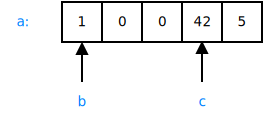
\includegraphics[width=0.7\textwidth]{figures/array.pdf}
  \end{column}
\end{columns}
\misc{
	\begin{itemize}
		\item Accessing a pointer as an array
		\item Pointer arithmetic according to array indexing
	\end{itemize}
	
	\textbf{Warning!} A pointer value is the byte address and types have different sizes which can be found using \ctext{sizeof(mytype)}.
}
\end{frame}
